\documentclass[a4paper,12pt]{article}
\usepackage{graphicx}

\usepackage{epstopdf}
\usepackage{gensymb}
\usepackage{float}
\usepackage{amssymb}
\usepackage{amsmath}
\usepackage{mathtools}
\usepackage{braket}
\usepackage{setspace}
\usepackage{tabularx}
\usepackage[htt]{hyphenat}
\title{Teknisk Dokumentation}
%% Definitioner för LIPS-dokument

\usepackage[swedish]{babel}
\usepackage[utf8]{inputenc}
\usepackage[T1]{fontenc}
\usepackage{times}
\usepackage{ifthen}
\usepackage[labelfont=it]{caption}

\usepackage[margin=25mm]{geometry}

\def\arraystretch{1.6}

\usepackage{fancyhdr}
\pagestyle{fancy}
\lhead{}
\chead{\LIPSprojekttitel}
\rhead{\LIPSdatum}
\lfoot{\LIPSkursnamn \\ \LIPSdokumentansvarig}
\rfoot{\LIPSprojektgrupp \\ \LIPSgruppepost}

\setlength{\parindent}{0pt}
\setlength{\parskip}{1ex plus 0.5ex minus 0.2ex}


\newcommand{\twodigit}[1]{\ifthenelse{#1<10}{0}{}{#1}}
\newcommand{\dagensdatum}{\number\year-\twodigit{\number\month}-\twodigit{\number\day}}

%% ------------------------------------------
% NYBILD
% Skapar centrerad bild med caption
%   
% #1: Filens url relativt '/bilder/'
% #2:  Caption
% #3: Label
% #4: Skalning i förhållande till textwidth
%% ------------------------------------------
\newcommand{\nyBild}[4] 
{\begin{figure}[H]
  \centering
 \emph{\includegraphics[angle=0,width=#4\textwidth]{bilder/#1}}
  \caption{\emph{#2}}
  \label{fig:#3}
\end{figure}}

%%  Redefinitions of commands containing @
\makeatletter
\makeatother

\newcommand{\LIPStitelsida}{%
{\ }\vspace{45mm}
\begin{center}
  \textbf{\Huge {\sffamily \LIPSdokumenttyp}}
\end{center}
\begin{center}
  {\Large \LIPSredaktor}
\end{center}
%\begin{center}
%  {\Large Version \LIPSversion}
%\end{center}
\vspace{60mm}
%\begin{center}
%  {\large Status}\\[1.5ex]
%  \begin{tabular}{|*{3}{p{40mm}|}}
%    \hline
%    Granskad & \LIPSgranskare & \LIPSgranskatdatum \\
%    \hline
%    Godkänd & \LIPSgodkannare & \LIPSgodkantdatum \\
%    \hline
%  \end{tabular}
%\end{center}
\newpage
}


\newenvironment{LIPSprojektidentitet}{%
{\ }\vspace{45mm}
\begin{center}
  {\Large PROJEKTIDENTITET}\\[0.5ex]
  {\small
  \LIPSprojektgrupp, \LIPSartaltermin, \LIPSprojekttitel\\
  Tekniska högskolan vid Linköpings universitet, ISY
  }
\end{center}
\begin{center}
  \begin{tabular}{|l|p{45mm}|p{25mm}|l|}
    \hline
    \textbf{Namn} & \textbf{Ansvar} & \textbf{Telefon} & \textbf{E-post} \\
    \hline
}
{
    \hline
  \end{tabular}
\end{center}
\begin{center}
  {\small
    \textbf{E-postlista för hela gruppen}: \LIPSgruppepost\\
    \textbf{Kontaktperson hos kund}: \LIPSkundkontakt\\
    \textbf{Kursansvarig}: \LIPSkursansvarig\\
    \textbf{Handledare}: \LIPShandledare\\
  }
\end{center}
\newpage
}
\newcommand{\LIPSgruppmedlem}[4]{\hline {#1} & {#2} & {#3} & {#4} \\}



\newenvironment{LIPSdokumenthistorik}{%
\begin{center}
  Dokumenthistorik\\[1ex]
  \begin{small}
    \begin{tabular}{|l|l|p{60mm}|l|l|}
      \hline
      \textbf{Version} & \textbf{Datum} & \textbf{Utförda förändringar} & \textbf{Utförda av} & \textbf{Granskad} \\
      }%
    {%
      \hline
    \end{tabular}
  \end{small}
\end{center}
}
\newcommand{\LIPSversionsinfo}[5]{\hline {#1} & {#2} & {#3} & {#4} & {#5} \\}



\newenvironment{packed_itemize}{
\begin{itemize}
	\setlength{\itemsep}{1pt}
    \setlength{\parskip}{0pt}
    \setlength{\parsep}{0pt}
}{\end{itemize}}

\newenvironment{packed_enumerate}{
\begin{enumerate}
	\setlength{\itemsep}{1pt}
    \setlength{\parskip}{0pt}
    \setlength{\parsep}{0pt}
}{\end{enumerate}}





%%% Local Variables: 
%%% mode: latex
%%% TeX-master: "kravspec_mall"
%%% End:

\usepackage{sectsty}
\allsectionsfont{\sffamily}

\frenchspacing

\renewcommand{\thepage}{\roman{page}}

\newcommand{\LIPSartaltermin}{VT14}
\newcommand{\LIPSkursnamn}{TSEA56 Elektronik kandidatprojekt}

\newcommand{\LIPSprojekttitel}{Lagerrobot}

\newcommand{\LIPSprojektgrupp}{Grupp 1}
\newcommand{\LIPSgruppepost}{tsea56-2014-grupp-1@googlegroups.com}
\newcommand{\LIPSdokumentansvarig}{LIPS Teknisk dokumentation}

\newcommand{\LIPSkund}{ISY, Linköpings universitet, 581\,83 Linköping}
\newcommand{\LIPSkundkontakt}{Tomas Svensson, 013-28 13 68, tomass@isy.liu.se}
\newcommand{\LIPSkursansvarig}{Tomas Svensson, 013-28 13 68, 3B:528, tomass@isy.liu.se}
\newcommand{\LIPShandledare}{Anders Nilsson, 3B:512, 013-28 26 35, anders.p.nilsson@liu.se}


\newcommand{\LIPSdokumenttyp}{Teknisk dokumentation}
\newcommand{\LIPSredaktor}{Karl Linderhed}
\newcommand{\LIPSversion}{1.0}
\newcommand{\LIPSdatum}{\dagensdatum}

\newcommand{\LIPSgranskare}{}
\newcommand{\LIPSgranskatdatum}{}
\newcommand{\LIPSgodkannare}{}
\newcommand{\LIPSgodkantdatum}{}

\setlength{\parskip}{\baselineskip}%
\setlength{\parindent}{0pt}%

\begin{document}

\LIPStitelsida

%% Argument till \LIPSgruppmedlem: namn, roll i gruppen, telefonnummer, epost
\begin{LIPSprojektidentitet}
  \LIPSgruppmedlem{Karl Linderhed}{Projektledare (PL)}{073-679 59 59}{karli315@student.liu.se}
  \LIPSgruppmedlem{Patrik Nyberg}{Dokumentansvarig (DOK)}{073 -049 59 90}{patny205@student.liu.se}
  \LIPSgruppmedlem{Johan Lind}{}{070-897 58 24}{johli887@student.liu.se}
  \LIPSgruppmedlem{Erik Nybom}{}{070-022 47 85}{eriny778@student.liu.se}
  \LIPSgruppmedlem{Andreas Runfalk}{}{070-564 23 79}{andru411@student.liu.se}
  \LIPSgruppmedlem{Philip Nilsson}{}{073-528 48 86}{phini326@student.liu.se}
  \LIPSgruppmedlem{Lucas Nilsson}{}{073-059 42 94}{lucni395@student.liu.se}
\end{LIPSprojektidentitet}


\renewcommand*\contentsname{Innehåll}
\begin{spacing}{0.5}
\tableofcontents{}
\end{spacing}
\newpage

%% Argument till \LIPSversionsinfo: versionsnummer, datum, ändringar, utfört av, granskat av
%\addcontentsline{toc}{section}{Dokumenthistorik}
\begin{LIPSdokumenthistorik}
  \LIPSversionsinfo{1.0}{2014-05-26}{Första version.}{KL}{Alla}
\end{LIPSdokumenthistorik}
\newpage

\renewcommand{\thepage}{\arabic{page}}
\setcounter{page}{1}

\section{Inledning}
Sju studenter vid Linköpings universitet har i sitt kandidatarbetsprojekt konstruerat en robot. Detta dokument tjänar till att vara ett underlag för någon som vill konstruera en liknande produkt och beskriver i detalj hur systemet fungerar.

\section{Produktbeskrivning}
Produkten är en robot bestående av ett chassi av plexiglas med fyra hjul, sensorer, en arm och styrelektronik. Utöver detta finns programvara för övervakning och manövrering av roboten.

Roboten är tänkt att användas i ett lager där den autonomt eller fjärrstyrt hämtar och lämnar lagervaror. Lagerarbetet utförs genom att följa en svart linje längs marken där stationer är markerade med ett svart sträck, vinkelrätt mot banan, i den riktning stationen befinner sig. Vid stationerna finns en RFID-tagg för identifiering av stationstypen, upplockning eller avlämning.

\section{Systemöversikt}
Roboten är uppbyggd av fyra olika delsystem kallade chassi, sensor, arm och kommunikation där var och en av dem har sin specifika uppgift att sköta. Förutom robotens fyra delsystem har programvara för persondatorer utvecklats för övervakning och styrning. Roboten kan både operera i ett fjärrstyrt, fullständigt manuellt, läge och i ett autonomt läge där möjligheten att styra vissa delar manuellt fortfarande ges.

\subsection{Delsystemsöversikt}
Sensorenheten övervakar kontinuerligt de för tillfället aktuella sensorerna och anpassar sensordata för tolkning av övriga delsystem.

Kommunikationsenheten fungerar som en förbindelselänk mellan roboten och omvärlden. Den hanterar kommunikationen mellan roboten och datorprogramvaran. Den förmedlar order, robotens status och sensordata. Vidare är kommunikationsenheten utrustad med en skärm som visar information från olika delsystem.

Chassienheten fungerar som det beslutande organet på roboten. Den vet vid autonomt läge hur roboten ska agera i olika situationer. Chassienheten samverkar med sensorenheten och ser till att roboten följer linjen, genom reglering av hjulens gaspådrag, baserat på den sensordata sensorenheten tillhandahåller. 

Armenheten kan vid en upplockningsstation, med vetskapen om var ett föremål befinner sig, plocka upp föremålet med robotarmen. Den har kontroll över samtliga servon i armen och vet hur dessa ska röras vid kommando. Med hjälp av inverterad kinematik kan den, vid automatiskt läge, beräkna hur vardera led ska röra sig för att nå föremålet och sedan plocka upp det.

Den datorbaserade programvaran består av ett instrumentbräde där användaren kan se vilka beslut som tas av roboten samt vilka sensordata de olika sensorerna får in. Vidare kan roboten, inklusive armen, styras genom kommandon i det grafiska gränssnittet.

\subsection{Sensorer och sensorplacering}

En linjesensor sitter längst fram på roboten, nära marken. En RFID-läsare sitter parallellt med och nära marken under roboten för att underlätta avläsning av RFID-taggar. På vardera sida av roboten är en avståndssensor monterad på ett servo, för att kunna svepa över ett område och skanna efter föremål att plocka upp.


\section{Gemensamma funktioner}
Detta avsnitt beskriver olika funktioner som inbegriper eller används av flera olika moduler.

\subsection{Protokoll för seriell kommunikation mellan robot och PC}
\label{sec:bt-protokoll}
Protokollet som roboten och PC-gränssnittet använder är uppbyggt av olika typer av paket. Varje typ av data som skickas har ett fördefinierat unikt paket-id, som indikerar för en mottagare hur datan ska hanteras. Paket-id:t är alltid den första byten av en överföring. Figur \ref{fig:btpaket} visar hur ett paket är uppbyggt.

\nyBild{Bluetooth-protokoll.png}{Ett paket i den seriella kommunikationen mellan robot och PC, varje ruta är en byte lång.}{btpaket}{0.8}

Paketlängden som skickas med är antalet parametrar + 1, eftersom även kontrollsumman ingår i paketet. Paketlängden indikerar alltså hur många bytes som finns kvar i paketet efter paketlängden.

Kontrollsumman bildas genom att summera värdena av alla bytes i paketet, exklusive kontrollsumman själv, trunkera summan till 8 bitar, och invertera värdet bitvis.

\begin{table}[H]
\begin{tabularx}{\textwidth}{|l|X|p{5cm}|}
\hline
\textbf{ID-beteckning} & \textbf{Beskrivning} & \textbf{Parametrar} \\ \hline
PKT\_STOP & Indikerar att roboten ska stoppa all rörelse. & Inga \\ \hline
\end{tabularx}
\caption{De olika pakettyper som kan skickas mellan roboten och PC och vad de innehåller. Parametrarnas ordningsnummer i parameterföljden anges inom parentes i den sista kolumnen.}
\end{table}

\subsection{USART}
\label{sec:usart}
AVR-processorns inbyggda USART-funktionalitet används av flera delsystem. Därför finns ett gemensamt bibliotek med funktionalitet för att skicka och ta emot byte över en seriell lina.

Biblioteket använder en byte-buffer för att lagra mottagen data. Till buffern hör två pekare, en läspekare och en skrivpekare, som pekar till olika element i buffern och flyttas upp när man läser eller skriver i buffern. Genom att pekarna endast kan anta värden mellan 0 och 255, samma antal värden som det finns element i buffern, fås funktionalitet som i en ringbuffer eftersom pekarnas värden svämmar över till 0 när de ökas från 255.

När avbrottet som indikerar att en byte har tagits emot skrivs den byte som har tagits emot in i buffern på den position som skrivpekaren pekar på. Därefter ökas pekarens värde ett steg.

\nyBild{USART-buffer.png}{Byte-buffern som USART-biblioteket använder, och vilken data som räknas som tillgänglig och ej ännu läst. En ruta föreställer en byte.}{usartbuffer}{0.6}

För att läsa en byte från buffern anropas funktionen \verb|usart_read_byte|. Den undersöker om det finns någon data tillgänglig som inte redan har lästs (med andra ord, om läs- och skrivpekaren skiljer sig från varandra, se figur \ref{fig:usartbuffer}). I annat fall väntar den tills dess att det finns data, dock som mest under en bestämd timeout-tid. När det finns data läser den in en byte från den position i buffern som läspekaren pekar på till en variabel, och stegar upp läspekaren med ett steg.

För att skicka data används funktionen \verb|usart_write_byte| som undersöker om den inbyggda USART-modulens statusflaggor tillåter att man skickar data, och i sådana fall ger funktionen en byte till USART-modulen som direkt matar ut den på den seriella linan. Går det inte att skicka väntar funktionen till dess att det går innan den skriver datan till USART-modulen.

\subsection{Intern buss}
\label{sec:bus}

För att delsystem internt ska kunna kommuicera med varandra finns en intern buss av typen multimaster I$^2$C\footnote{Inter-Integrated Circuit, en synkron seriell multimasterbuss.} implementerad.

\subsubsection{Protokoll}
\label{sec:bus-protokoll}
Alla transaktioner består utav en adress med en skriv- eller läsbit, följt av två bytes med data. Då enheten som initierat kontakten (master) vill skriva ut på bussen består de första 5 bitarna av ett id. Detta id bestämmer vilken funktion hos slaven som ska hantera den data som överförs i de resterande 11 bitarna.

\nyBild{Buss-protokoll.pdf}{En lyckad skrivning från master till slav. Om NACK skulle ha returnerats istället för ACK kommer överföringen att avbrytas.}{busstransaktion}{1}

I fallet att master vill göra en förfrågan på bussen gör den först en skrivning till slaven. Detta gör då att slaven kör funktionen på det id den fick med de resterande 11 bitar som inargument. Denna funktion returnerar ett 16 bitars värde vilket kommer vara det värde som skickas ut då mastern sedan begär en läsning från slaven. Mellan dessa två transaktioner är det viktigt att mastern inte släpper kontroll över bussen, eftersom slaven då skulle kunna returnera fel värde om en annan enhet skrivit till den efter den första transaktionen.

\subsubsection{Implementation}
\label{sec:bus-implementation}
Bussen är implementeras så att alla enheter kan initiera en transaktion och därmed kan alla enheter vara master på bussen. Detta gör att två eller fler enheter kan börja kommunicera på bussen samtidigt. Då detta sker kommer den enhet som skickar en låg bit först att vinna bussen och fortsätta med sin transaktion. De andra enheterna kommer då upphöra med sina transaktioner och efter att ett stop skickats på bussen kommer de att försöka igen. Detta kommer enheterna att göra tills dessa att de lyckats med en transaktion.

\begin{table}[H]
\centering
\label{adress-buss}
\begin{tabularx}{0.5\textwidth}{|X|X|}
\hline
\textbf{Enhet} & \textbf{Adress} \\ \hline
Sensor & 4 \\ \hline
Kommunikation & 5 \\ \hline
Chassi & 1 \\ \hline
Arm & 6 \\ \hline
\end{tabularx}
\caption{Adresser till de olika delsystem på den interna bussen.}
\end{table}

När en enhet gör en transaktion på bussen och enheten som tar emot data returnerar NACK (no acknowledgement) efter någon byte i överförningen kommer transaktionen att avbrytas och en ny kommer inte att startas.

För att bestämma vilken funktion som ska hantera data på vilket id finns funktionerna \verb|bus_register_receive|, som registrerar en funktion för mottagen data, samt \verb|bus_register_response| som registrerar en funktion då data ska returneras över bussen. 

Funktionen för att skicka data på bussen är \verb|bus_transmitt|, och för att göra en förfrågan finns \verb|bus_request|. Båda dessa returnerar 0 då transaktionen lyckades. Detta innebär att om användaren vill vara säker på att en transaktion ska gå fram på bussen måste dessa funktioner köras tills dess att de returnerar 0.

Hastigheten på bussen har valts till så låg som möjligt, detta för att få maximal stabilitet. Eftersom hastigheten sätts genom en division av klockhastigheten till processorn kommer bussen att gå olika fort beroende av vilken enhet som är master. Detta innebär att hastigheten varierar mellan cirka 70 och 90 kHz.

\subsection{Utmatning på LCD-skärm}
\label{sec:lcd_interface}

Alla enheter kan mata ut information på kommunikationsenhetens LCD-skärm. Detta görs genom biblioteket \verb|lcd_interface| och funktionen \verb|display|. Funktionen kan ta godtyckligt antal parametrar, dock som minst två där den första anger vilken av LCD-skärmens två rader man vill använda och den andra är en sträng med texten som ska skrivas ut. Övriga parametrar är variabler som man vill mata ut, dessa refereras till i textsträngen med samma syntax som är standard i funktionen \verb|printf| i C.

LCD-skärmen kommer att rotera mellan de fyra olika enheternas meddelanden med ca två sekunders intervall. Varje ''sida'' som visas på skärmen identifieras med en bokstav för vilken enhet som visas för tillfället: ''C'' för chassienheten, ''S'' för sensorenheten, ''K'' för kommunikationsenheten och ''A'' för armenheten.

\section{Kommunikationsenhet}
Kommunikationsenheten är robotens gränssnitt för interaktion med omvärlden och har två uppgifter. Den ska
\begin{itemize}
\item agera som ett gränssnitt mot LCD-skärmen och möjliggöra att alla delsystem kan skriva ut information på den.
\item hantera den seriella kommunikationen över blåtand och möjliggöra att roboten kan skicka och ta emot information till och från PC-gränssnittet.
\end{itemize}

Figur \ref{fig:kommblock} ger en övergripande bild över kommunikationsenhetens beståndsdelar.

\nyBild{Block-komm.png}{Blockschema över kommunikationsenheten.}{kommblock}{0.9}

\subsection{LCD-gränssnitt}
LCD-skärmen som är monterad på kommunikationsenheten är av modellen JM162A. Den styrs genom en parallell databuss och ett antal styrsignaler från kommunikationsenhetens processor till en intern processor i LCD-enheten. Skärmen har två rader med 16 tecken vardera. \cite{lcd}

Information skickas till LCD-enheten antingen som instruktioner eller data. Styrsignalernas koppling visas i figur \ref{fig:kommblock}. \verb|RS| styr om databussens värde tolkas som instruktion eller data, \verb|R/W| styr ifall information ska skrivas eller läsas, och styrsignalen \verb|E| aktiverar överföring av information. Genom att låta \verb|E| gå från hög till låg läser LCD-enheten in värdet som finns på databussen, antingen som en instruktion som ska utföras (om \verb|RS| är låg) eller som data som ska lagras i LCD-enhetens minne (om \verb|RS| är hög). Figur \ref{fig:lcdinit} visar vilka kommandon som skickas för att initiera LCD-enheten.

\nyBild{lcd-init.png}{Flödesschema över initialisering av LCD-enhet. Kommandon som skickas är kursiverade och har värdena på DB (i binär notation), RS och R/W som parametrar.}{lcdinit}{0.4}

Efter denna initiering kan data skrivas ut på skärmen genom att sätta \verb|RS| till 1 och skriva ut ASCII-koden\footnote{American Standard Code for Information Interchange, ett sätt att koda grundläggande alfanumeriska tecken och andra symboler.} för en symbol på databussen. Genom att först skicka en instruktion för att ställa in vilken adress i dataminnet som ska skrivas till härnäst kan man välja var en symbol ska skrivas ut, en viss adress i dataminnet svarar mot en position på skärmen.

Alla delsystem kan skriva ut information på skärmen genom ett gemensamt bibliotek, \textit{lcd\_interface}, som beskrivs närmare i avsnitt \ref{sec:lcd_interface}.


\subsection{Seriell kommunikation över blåtand}
Anslutningen till datorn sker med blåtandsmodemet \emph{BlueSMiRF Gold} som är monterat på roboten \cite{bluetooth}. På PC-sidan skapas vid parkoppling med modemet en virtuell serieport, som emulerar en fysisk COM-port eller motsvarande. Kommunikationen sker sedan över denna port som om den vore en vanlig RS-232-port\footnote{RS-232 är en typ av seriell kommunikation vid överföring av data \cite{rs232}.}. 

På robotsidan används AVR-processorns inbyggda modul för USART, och det gemensamma biblioteket för USART som används av flera delsystem -- se avsnitt \ref{sec:usart}. Följande parametrar ställs in i det protokoll som roboten använder:
\begin{itemize}
\item Datahastigheten är 115 200 bps.
\item Data skickas som 8-bitars värden utan någon paritetsbit.
\item Ingen flödeshantering eller handskakning används.
\item Varje värde om 8 bitar avslutas med en stoppbit.
\end{itemize}

Hur olika typer av information överförs mellan robot och PC beskrivs närmare i avsnitt \ref{sec:bt-protokoll}.

\section{Sensorenhet}
Sensorenhetens uppgift är att samla in rådata från de olika sensorerna och formatera denna till information som är användbar för robotens övriga delsystem. På begäran av andra delsystem skickar sensorenheten ut data via bussen. Sensorenheten är utrustad
med en linjesensor vars uppgift är att ge information om robotens position i förhållande till tejplinjen. Informationen används som styrdata och skickas över bussen i form av en tyngdpunkt till chassimodulen för styrreglering.

Vidare är roboten utrustad med två sidoskannrar, en på vardera sida. Dessa används för att lokalisera föremålet roboten ska plocka upp. Om ett föremål hittas räknar sensorenheten ut en koordinat för föremålet och skickar koordinaten över bussen till armenheten.


\subsection{Sensorer}
Sensorenheten använder tre olika sensortyper: avståndssensor, linjesensor och RFID-läsare.
Dessa beskrivs kortfattat nedan. En djupare beskrivning av hur komponenterna fungerar finns i bilaga sensorfördjupning.

\subsubsection{Avståndssensorer}
Avståndssensorerna används till robotens sidoskannrar. De mäter avstånd genom att skicka ut infrarött ljus som sedan reflekteras tillbaka i en PSD, Position Sensitive Detector. Avståndssensorerna som används fungerar för avstånd mellan \mbox{$4-30$ cm}. Eftersom de först mäter ett digitalt värde och sedan skickar ut en analog spänning uppstår brus på utsignalen. Detta brus är relativt högfrekvent varför det filtreras bort med hjälp av ett lågpassfilter innan signalen når processorn. Se kopplingsschema, figur \ref{fig:senskoppling}.

En avläsning från en avståndssensor görs genom att omvandla sensorns analoga utspänning till ett digitalt värde. När A/D-omvandlingen är klar jämförs den A/D-omvandlade spänningen med en tabell över kända avstånd och spänningar för att översätta denna till ett avstånd i millimeter. Värden som inte finns i tabellen beräknas med linjärinterpolering. 

Avståndssensorerna är, inom det intervall de är designade att arbeta, kapabla till att uppnå hög precision men olika föremål kan få avståndssensorn att ge ut olika spänningar för samma avstånd. Detta leder till att det är av stor vikt att alla avståndssensorer kalibreras i den miljö de är tänkta att användas. Kalibreringen sker genom att identifiera vilka spänningar som svarar mot kända avstånd och föra in dessa som konstanter i sensorenhetens programkod. Avståndssensorerna har även ett område inom vilket de klarar av att känna av avstånd. Detta område breder huvudsakligen ut sig i horisontell led. Detta har på roboten tagits i beaktning genom att montera de avståndssensorer som sitter på sidoskannrarna vertikalt snarare än horisontellt.

\subsubsection{Linjesensor}
\label{sec:linjesensor}
Reflexsensormodulen består av en uppsättning IR-dioder och fototransistorer som tillsammans används för att mäta reflektionsförmågan hos underlaget. Eftersom reflexsensormodulen består av 11~stycken separata IR-dioder och fototransistorer används en multiplexer och en demultiplexer för att styra sensorn. Demultiplexern driver IR-dioderna och multiplexern används för att ta in insignalerna från fototransistorerna. Linjesensorn är kopplad i enlighet med kopplingsschemat i figur \ref{fig:senskoppling}.

Reflexsensorn ger ut en analog spänning som är omvänt proportionell mot underlagets reflekterande ljusstyrka. En inläsning från linjesensorn sker genom ett funktionsanrop till linjesensorinläsningsfunktionen som finns på sensorenheten. När denna funktion anropas uppdateras en uppsättning variabler som är lagrade i en vektor. Vektorn är 11 element lång, där varje element representerar en reflexsensor.

När uppdateringen av linjesensorn startas för första gången är multiplexrarna som styr linjesensorn inställda så att reflexsensorn längst till vänster väljs. Efter detta startas A/D-omvandling på kanal~0 som svarar mot den pinne på processorn som reflexsensormodulen är kopplad till. Under vidare körning så påbörjas varje uppdatering av reflexsensorerna med att en A/D-omvandling startas varefter programmet väntar på att omvandlingen ska slutföras. När A/D-omvandlingen är färdig läggs sedan det erhållna värdet in i linjesensorns datavektor.


\subsubsection{RFID-läsare}
Den RFID-läsare som används är en “Parallax Serial”. Denna kräver två pinnar på processorn enligt kopplingsschema i figur \ref{fig:senskoppling}. När chassit har stannat på en station beordras sensorenheten att göra en RFID-läsning. Då körs ett program på sensorenheten som aktiverar läsaren, rensar läsarbufferten och sedan väntar programmet på att en inläsning sker, vilket i regel tar cirka 150 - 300 ms. Läsaren kommunicerar med sensorenhetens processor via USART och så fort antennen låst sig på en tagg skickas värdet till processorn där det lagras i en buffert. Så fort det finns data i bufferten väntar programmet ytterligare 50 ms för att all data ska hinna läsas in till bufferten från RFID-taggen innan avläsning av bufferten sker. Sedan jämförs det inlästa värdet med RFID-taggar som redan finns lagrade i processorns minne. Om någon av de redan lagrade taggarna matchar det inlästa värdet skickar sensorenheten tillbaka den siffra som står på motsvarande RFID-tagg. Om ingen inläsning gjorts innan 400 ms ger programmet upp och skickar till chassienheten att inget hittades.

\subsection{Sidoskanner}
Sidoskannerns uppgift är att hitta det objekt som ska plockas upp när roboten har stannat vid en plockstation. Sidoskannern består av två avståndssensorer, på höger respektive vänster sida om roboten, monterade på varsitt servo. Servona styrs med hjälp av pulsbreddsmodulering. Servot får en puls var 20:e~ms och pulsbredden avgör vilket läge servot antar. En pulsbredd på ungefär 0.5~ms motsvarar servots minsta utslag och en pulsbredd på ungefär 2.5~ms motsvarar max vinkelutslag. Värden på dessa utslag varierar dock något från servo till servo.

För att få ett servot att svepa över robotens ena sida ökas pulsbredden inkrementellt med en stegkonstant motsvarande ett servoutslag på en grad. För varje iteration, dvs. för varje vinkel servot står i, kommer avståndssensorn lägga in 20 stycken A/D-omvandlade avståndsmätningar i en array för att sedan ta medianvärdet av mätningarna. Detta görs för att bli av med eventuella avvikande värden som fås ur avståndssensorerna. Slutligen omvandlas värdet till ett avstånd i millimeter genom att interpolera mellan de olika referensvärden som finns lagrade i processorn. Om avståndet är större än vad armens räckvidd är innebär det att att inget föremål detekterats och servots vinkel stegas upp ytterligare en grad. 

När avståndssensorn däremot påträffar ett föremål inom armens räckvidd sparas både vinkeln som servot står i och avståndet till föremålet undan innan sidoskannern stegar upp igen. För varje vinkel som avståndssensorerna fortfarande träffar föremålet sparas avståndet undan och slutligen även den sista vinkeln då den fortfarande träffade ett föremål.

Den vinkel som föremålet slutligen beräknas stå i ligger mitt emellan den första och sista vinkeln där föremålet detekterats. Vidare beräknas avståndet till föremålet som medianen av de mätningar som gjordes under tiden föremålet detekterats. Detta görs för att minimera den inverkan som kraftigt avvikande värden annars skulle kunna få. Medelvinkeln $\alpha$ och medianavståndet $L$ används sedan för att beräkna en koordinat utifrån vilken armen kan plocka upp föremålet. Denna koordinat är planpolär och består således av en vinkel $\beta$ och ett avstånd, $R$. Här är $\beta$ den vinkel som basplattan ska stå i för att armen ska vara riktad mot föremålet och $R$ är avståndet från robotens mittpunkt ut till föremålet. Se figur \ref{fig:sidoskanner}
\nyBild{sidoskanner.png}{Vänster sidoskanner.}{sidoskanner}{0.7}


\subsubsection{Koordinatberäkning}
När sidoskannern har hittat ett objekt och med flera mätningar noggrant identifierat avståndet $L$ och vinkeln $\alpha$ används dessa för att räkna ut $R$ och $\beta$ genom att kalla på två funktioner, \texttt{calculate\_angle\_coordinate} och \texttt{calculate\_distance\_coordinate}.
Vid montering av sidoskannrarna mäts avståndet från robotens origo, dvs. armens mittpunkt, till servonas rotationsaxel, se figur \ref{fig:sidoskanner}. Avståndet definieras som konstanten Origo-to-scanner-distance och används i koordinatberäkningsfunktionerna.

En temporär koordinat för objektet i förhållande till origo bestäms:
$$\begin{pmatrix}
x \\ y
\end{pmatrix}
 = 
\begin{pmatrix}
Konstant+L \sin(\alpha) \\ 
L \cos(\alpha)
\end{pmatrix}$$

Sen fås $R$ och $\beta$:
$$\begin{pmatrix}
R \\ \beta
\end{pmatrix}
 = 
\begin{pmatrix}
\sqrt{x^2 + y^2} \\ 
\arctan(\frac{x}{y})
\end{pmatrix}$$

\subsection{Linjeföljning}
Linjeföljning är en central del i robotens förmåga att utföra sitt uppdrag. Nedan beskrivs de väsentliga delar som ingår i denna process. Inläsning från linjesensorn beskrivs i \ref{sec:linjesensor}.

\subsubsection{Korsning, avbrott och plockstationsdetektering}

Plockstationsdetektering sker genom att roboten först och främst kontrollerar huruvida linjesensorn registrerar tejp utöver den tejpade linjen. Ifall att de fyra sensorerna längst ut antingen till höger eller vänster på reflexsensormodulen indikerar tejp innebär detta att vi antingen är vid en plockstation eller vid en korsning. Först när det har skett 2000 A/D-omvandlingar kommer roboten att stanna på en plockstation. Under denna tid kommer roboten fortlöpande att kontrollera huruvida linjesensorn registrerar tejp på den andra sidan om roboten. På detta sätt säkerställs att roboten inte stannar vid korsningar. Om den å andra sidan registrerar tejp på andra sidan också innebär det korsning och den kan köra vidare. 

För att hantera avbrott i tejplinjen kontrolleras fortlöpande huruvida roboten är över en linje. I det fall att roboten tappar linjen helt och hållet så kommer den utifrån sensorenheten skickade tyngdpunkten att vara 127, vilket motsvarar att linjen ligger på mitten. Eftersom att avbrott i tejpen i enlighet med banspecifikationen som längst får vara 10 centimeter långa är detta tillvägagångssätt fullt tillräckligt för att hantera avbrott i tejpen.
 
%\nyBild{programfl_de-_sensorenheten_uppdaterar_variabler.jpg}{Programflöde för att upptäcka korsning eller plockstation}{senskorsning}{0.8}


\subsubsection{Tyngdpunktsberäkning}
För att roboten ska känna till sin egen position i förhållande till linjen så ses de värden som registreras av de individuella sensorerna på reflexsensorn som tyngder. Ett högre värde motsvarar en större tyngd. De olika tyngder som finns på linjesensorn används sedan för att beräkna en tyngdpunkt hos linjesensorn. Eftersom att de reflexsensorer som läser av tejpen kommer att väga betydligt mer än de som läser av golvet kommer tejpen alltid att finnas där tyngdpunkten beräknas ligga hos linjesensorn.

Tyngdpunktsberäkningen använder sig av två stycken variabler. Den första variabeln innehåller linjesensorns totalvikt, alltså summan av de individuella reflexsensorernas värden. Den andra variabeln innehåller sensorns totalvikt, men där de olika reflexsensorerna även har blivit multiplicerade med en skalfaktor. Denna skalfaktor fyller två funktioner. Först och främst behövs den för att ge sensorerna på kanterna en större hävarm relativt linjesensorns mittpunkt. Vidare används den till att skala den slutgiltiga tyngdpunkten så att hela talområdet hos det åtta bitar stora returvärdet används för att representera linjen. Denna metod kommer att resultera i att tyngdpunkten representeras av ett åtta bitar stort heltalsvärde.

Då tyngdpunkten är 0 ligger tejpen alltså längst till vänster på reflexsensorn på samma sätt som en mekanisk tyngdpunkt hade legat längs till vänster om all massa hos en linje hade legat till vänster. Motsvarande innebär tyngdpunkt 255 att linjen ligger längs ut till höger på linjesensorn.








\section{Chassienhet}
\emph{Det här avsnittet ska innehålla mera detaljerade blockscheman och beskrivningar av modulen.
Tänk på läsbarheten och växla mellan figurer och text.}
\section{Armenhet}

Robotens arm är av modell PhantomX Reactor från Trossen Robotics, som är en servostyrd arm med 4 rotationsleder och en griphand varpå det sitter totalt 7~st AX-12A-servon. Armen kontrolleras av en microprocessor, ATmega 1284, genom att parallellkoppla servona till en seriell UART-port. Kommunikationen till servona sker via half duplex via en tri state buffer. Armen har en maximal räckvidd på 38~cm och en bas med  300~grader rotationsfrihet.

\subsection{Funktion}

Armen kan styras manuellt via PC-programvaran och kan köras i autonomt läge. Enhetens huvudprogram är avvaktande tills dess att kommando skickas till enheten vilket kan antingen vara ett manuellt styrningskommando eller en order från chassienheten att ta hand om upplockning av objekt.

\subsubsection{Manuellt läge} 

Vid manuellt läge får armen ingen upplockningsorder från chassienheten och väntar därför endast efter ett styrkommando från PC. Från PC får den ett kommando att röra sig i en viss riktning i koordinatsystemet visat i figur \ref{fig:arminverskinematik}.

Användaren kan välja att röra armen i djupled (Y-axeln), i höjd (Z-axeln), rotera runt Z-axeln eller öppna och stänga klon. Vid ett styrkommando rör sig armen i den angivna riktningen tills dess att ett kommando om att stanna rörelse i den riktingen ges från PC eller om den nått max-läget. Rörelse görs genom att kontinuerligt beräkna hur vinkeln av vardera led på armen skall ändras för att röra sig ett litet steg i den beordrade riktningen, detta görs genom beräkningar i inverterad kinematik (se \ref{inverskinematik}), sedan gör lederna en vinkelförändring för att sedan repetera enligt ovan.

Armen kan också via PC automatiskt röra sig till ett förbestämt läge, ett startläge, där rörelsen även här beräknas med inverterad kinematik till den position som startläget har. Först rör sig armen rakt upp från det nuvarande läget för att sedan röra sig till den position som startläget har, detta för att eliminera risken att stöta i chassit och virkorten.

\subsubsection{Autonomt läge}

Vid autonomt läge avvaktar armenheten tills dess att chassit har identifierat att vi befinner oss på en plockstation som är aktuell för upplockning eller avlämning. Vid station får armenheten en order, plocka upp eller lämna av objekt till höger eller till vänster. När ordern inkommer och armen inte redan håller i ett föremål tillkallar den sensorenheten att med, beroende på vilken sida stationen befinner sig på, en av sidoscannrarna söka igenom upplockningszonen. Håller armen redan i ett föremål rör den sig till samma koordinat som för upplockningen av samma objekt, släpper föremålet och rör sig sedan tillbaka till startläget för att sist skicka bekräftelse till chassit med status om avlämning lyckats.

Sensorenheten kommer, när den är klar med sidoscannrarna, skicka tillbaka ett kommando till armenheten med en vinkel och ett avstånd till föremålet, om den hittat något, annars meddelar den att zonen är tom. Med vinkeln och avståndet beräknar armenheten först en koordinat till objektet och sedan, med inverterad kinematik, hur armens olika leder behöver röra på sig för att nå koordinaten. Armen rör sig sedan mot objektet och väntar på att servona ska nå slutdestinationen, genom att fråga servona om de rör på sig, för att sedan gripa tag och röra sig tillbaka till startläget. Armenheten sparar sedan koordinaten där den plockat upp föremål, vilket används som avlämningsposition, och skickar bekräftelse till chassienheten om att upplockning av föremål lyckats. 

\subsubsection{Inverterad kinematik}
\label{inverskinematik}

Från sensorenheten ges armenheten en planpolär koordinat för objektet, dvs ett avstånd till föremålet och en vinkel för bottenplattan. Inverterad kinematik innebär att utifrån givna koordinater bestämma vinklar på robotarmens leder för att få armens spets att nå den givna koordinaten. För att reducera problemets komplexitet kunde armen, utifrån den givna vinkeln, ställa in sig mot föremålet och således förenkla det inverterade kinematikproblemet till ett tvådimensionellt sådant.

Problemet som kvarstod blev således att utifrån tre ihopsatta leder finna en lösning för ledvinklarna så att spetsen av kedjan, gripklon, hamnar på den kända positionen för föremålet. Se figur \ref{fig:inv_kin}

\nyBild{arm_figure.pdf}{2-dimensionell schematisk beskrivning över armen och dess leder.}{inv_kin}{0.7}

Genom att betrakta figur \ref{fig:inv_kin} som ett koordinatsystem med en $x$- och en $y$-axel ges gripklons position enligt ekvation \ref{eq:angle_to_coords}.

\begin{equation}
	\label{eq:angle_to_coords}
	f(\boldsymbol{\alpha})
	=
	\begin{pmatrix}
		L_{1}cos(\alpha_{1}) + L_{2}cos(\alpha_{1} + \alpha_{2}) + L_{3}cos(\alpha_{1} + \alpha_{2} + \alpha_{3})\\
		L_{1}sin(\alpha_{1}) + L_{2}sin(\alpha_{1} + \alpha_{2}) + L_{3}sin(\alpha_{1} + \alpha_{2} + \alpha_{3})
	\end{pmatrix}
	=
	\begin{pmatrix}
		T_x \\
		T_y
	\end{pmatrix}
	,
	\boldsymbol{\alpha}
	\in
	\mathbf{A}
\end{equation}

$f(\boldsymbol{\alpha})$ har en definitionsmängd $\mathbf{A}$ enligt ekvation \ref{eq:angle_to_coords_domain}. Bivillkoren i mängden $\mathbf{A}$ kommer direkt ifrån robotarmens datablad.

\begin{equation}
	\label{eq:angle_to_coords_domain}
	\mathbf{A}
	=
	\Set{
		\boldsymbol{\alpha} \in \mathbb{R}^{3} :
			0 \leq \alpha_1 \leq \pi,
			-\pi \leq \alpha_2 \leq 0,
			\frac{-\pi}{2} \leq \alpha_3 \leq \frac{\pi}{2}}
\end{equation}

Målet är att finna en funktion $f^{-1}(x, y) = \boldsymbol{\alpha}$, vilket inte är helt lätt för tre leder.

Först väljs $P$ någonstans längs cirkelperiferin runt $T$ med $L_3$ som radie. Valet kommer med fördel alltid ligga på samma höjd som $T$, vilket resulterar i att $L_3$ hålls parallell underlaget, såvida punkten $P$ inte krockar med roboten. Med en känd koordinat $P$ kan vinklarna $\alpha_{1}$ och $\alpha_{2}$ bestämas genom att lösa ekvationssystemet, se ekvation \ref{eq:theta1_linear_eq_solution}. För härledning av ekvationen, se bilaga XX

\begin{equation}
	\label{eq:theta1_linear_eq_solution}
	\begin{pmatrix}
		cos(\alpha_{1})\\
		sin(\alpha_{1})
	\end{pmatrix}
	=
	\frac{1}{L_1^2 + L_2^2 + 2 L_2 cos(\alpha_{2})}
	\begin{pmatrix}
		L_1 + L_2 cos(\alpha_{2}) & L_2 sin(\alpha_{2})\\
		-L_2 sin(\alpha_{2}) & L_1 + L_2 cos(\alpha_{2})
	\end{pmatrix}
	\begin{pmatrix}
		P_x \\
		P_y
	\end{pmatrix}
\end{equation}

När sinus- och cosinusvärdena är kända för både $\alpha_{1}$ och $\alpha_{2}$ kan den teckenkänsliga funktionen $atan2$ användas för att räkna ut vinklarna enligt ekvation \ref{eq:theta_p_solution}.

\begin{equation}
	\label{eq:theta_p_solution}
	\begin{pmatrix}
		\alpha_{1}\\
		\alpha_{2}
	\end{pmatrix}
	=
	\begin{pmatrix}
		atan2(sin(\alpha_{1}), cos(\alpha_{1}))\\
		atan2(sin(\alpha_{2}), cos(\alpha_{2}))
	\end{pmatrix}
\end{equation}

Eftersom $sin(\alpha_{2})$ har två lösningar uppstår således dubbla lösningar till ekvationssystemet. Därför är det viktigt att stämma av resultatet mot definitionsmängden $\mathbf{A}$.

Väl punkten $P$ och $T$ samt vinklarna $\alpha_{1}$ och $\alpha_{2}$ är kända ges $\alpha_{3}$ enligt ekvation \ref{eq:calc_alpha3}. Därmed är beräkningarna klara.

\begin{equation}
	\label{eq:calc_alpha3}
\alpha_{3} = atan2(sin(T_y - P_y), cos(T_x - P_x)) - \alpha_{2} - \alpha_{1}
\end{equation}

\subsection{Kopplingsschema}
%\nyBild{kopplingsschema-arm}{Kopplingsschema över delsystem arm}{kopparm}{1}

\subsection{Komponenter}

\begin{packed_itemize}
\item 1 x PhantomX Reactor arm med 7st AX-12A-servon
\item 1 x 3-state buffer (74LS241)
\item 1 x ATMega1284P, huvudprocessor
\item 1 x EXO-3, kristalloscillator (16~MHz)
\item 1 x Knapp med Resistor, för pullup av reset
\item 1 x Kondensator, för fördröjning av resetpullup vid start
\end{packed_itemize}

\subsection{Översiktlig beskrivning av programmet}

Programmet kommunicerar med servona över UART via funktioner som finns i ett delat bibliotek för denna typ av kommunikation. Servona styrs genom att skriva på deras minnen, där en skrivning på särskilld plats i minnet leder till en särskilld instruktion till servot. För att skriva eller läsa från servona skapas i programmet först ett paket, med utseende beroende på instruktion, med samtliga bitar som ska skickas för att sedan seriellt skicka dem via UART. Vid en överföring, borstett från när instruktion skickas till alla servon, väntar programmet på att få svar från servot för att kunna diagnostisera om instruktionen kunnat genomföras eller för att tyda en avläsning av servominne. Svar omhändertas genom väntan på mottagningsavbrott på armenheten därpå inkommande data lagras i en mottagningsbuffer som läses av så fort den inte är tom.

Eftersom armenheten är avvaktande utför huvudprogrammet endast instruktioner när statusflaggor blivit satta genom funktionskallelser från andra enheter på bussen. 

Med hjälp av inverterad kinematik kan programmet beräkna vilka vinklar armens servon ska anta för att armens gripklo ska anta en given position.

Nedanstående figur visar vilka bibliotek som programmet består av. Grönmarkerade lådor innebär att de kan delas med andra delar av roboten. Lådor som ligger ovanför en annan låda bygger på den lådans funktioner. Exempelvis är servostyrning och servoläsning beroende av funktioner för att kommunicera över UART.

%\nyBild{Programstruktur_arm.png}{Övergripande bild över armenhetens programbibliotek.}{armprogrambibliotek}{0.8}
\section{Programvara till persondator}
Programvaran till persondatorer som finns till roboten är till dels för att ge kommandon till roboten, och dels för att visa utmatning av sensordata och beslut. För användning, se användar manualen.

Programvaran är utvecklad i utvecklingsmiljön Qt, och använder till stor del Qt:s egna standard bibliotek. Den är uppdelad i två klasser, en för att kommunicera med roboten via blåtand och en för det grafiska interfacet.

Klassen för blåtands kommunikation använder sig utav QSerialPort, vilket finns i Qt:s standard bibliotek. Ur detta hanterar klassen när data ska skickas och tas emot från roboten, och vidarebefordrar denna data till klassen som sköter det grafiska.

Klassen för det grafiska interfacet innehåller alla knappar, fält och liknande som finns i det grafiska interfacet. Denna använder också till stor del Qt:s egna standard bibliotek. Detta gör att klassen till största del innehåller vad de olika knapparna ska göra då de klickas på. Detta består i de flesta fall av att skicka ett visst packet till roboten.

I det grafiska interfacet finns också två grafer som ritar ut data från linjesensorn samt sidoskannrar. Dessa använder en klass som heter QCustomPlot, för ytterligare beskrivning se \ref{}.  

\newpage
\section*{Referenser}


\newpage
\appendix
\section{Kopplingsschema}
Robotens elektronik är uppdelad på två virkort. Därför presenteras här ett kopplingsschema för varje virkort.


\nyBild{kopplingsschema_sensor.pdf}{Kopplingsschema för virkortet som innehåller sensorenheten.}{senskoppling}{1}

\begin{figure}[H]
\centering
 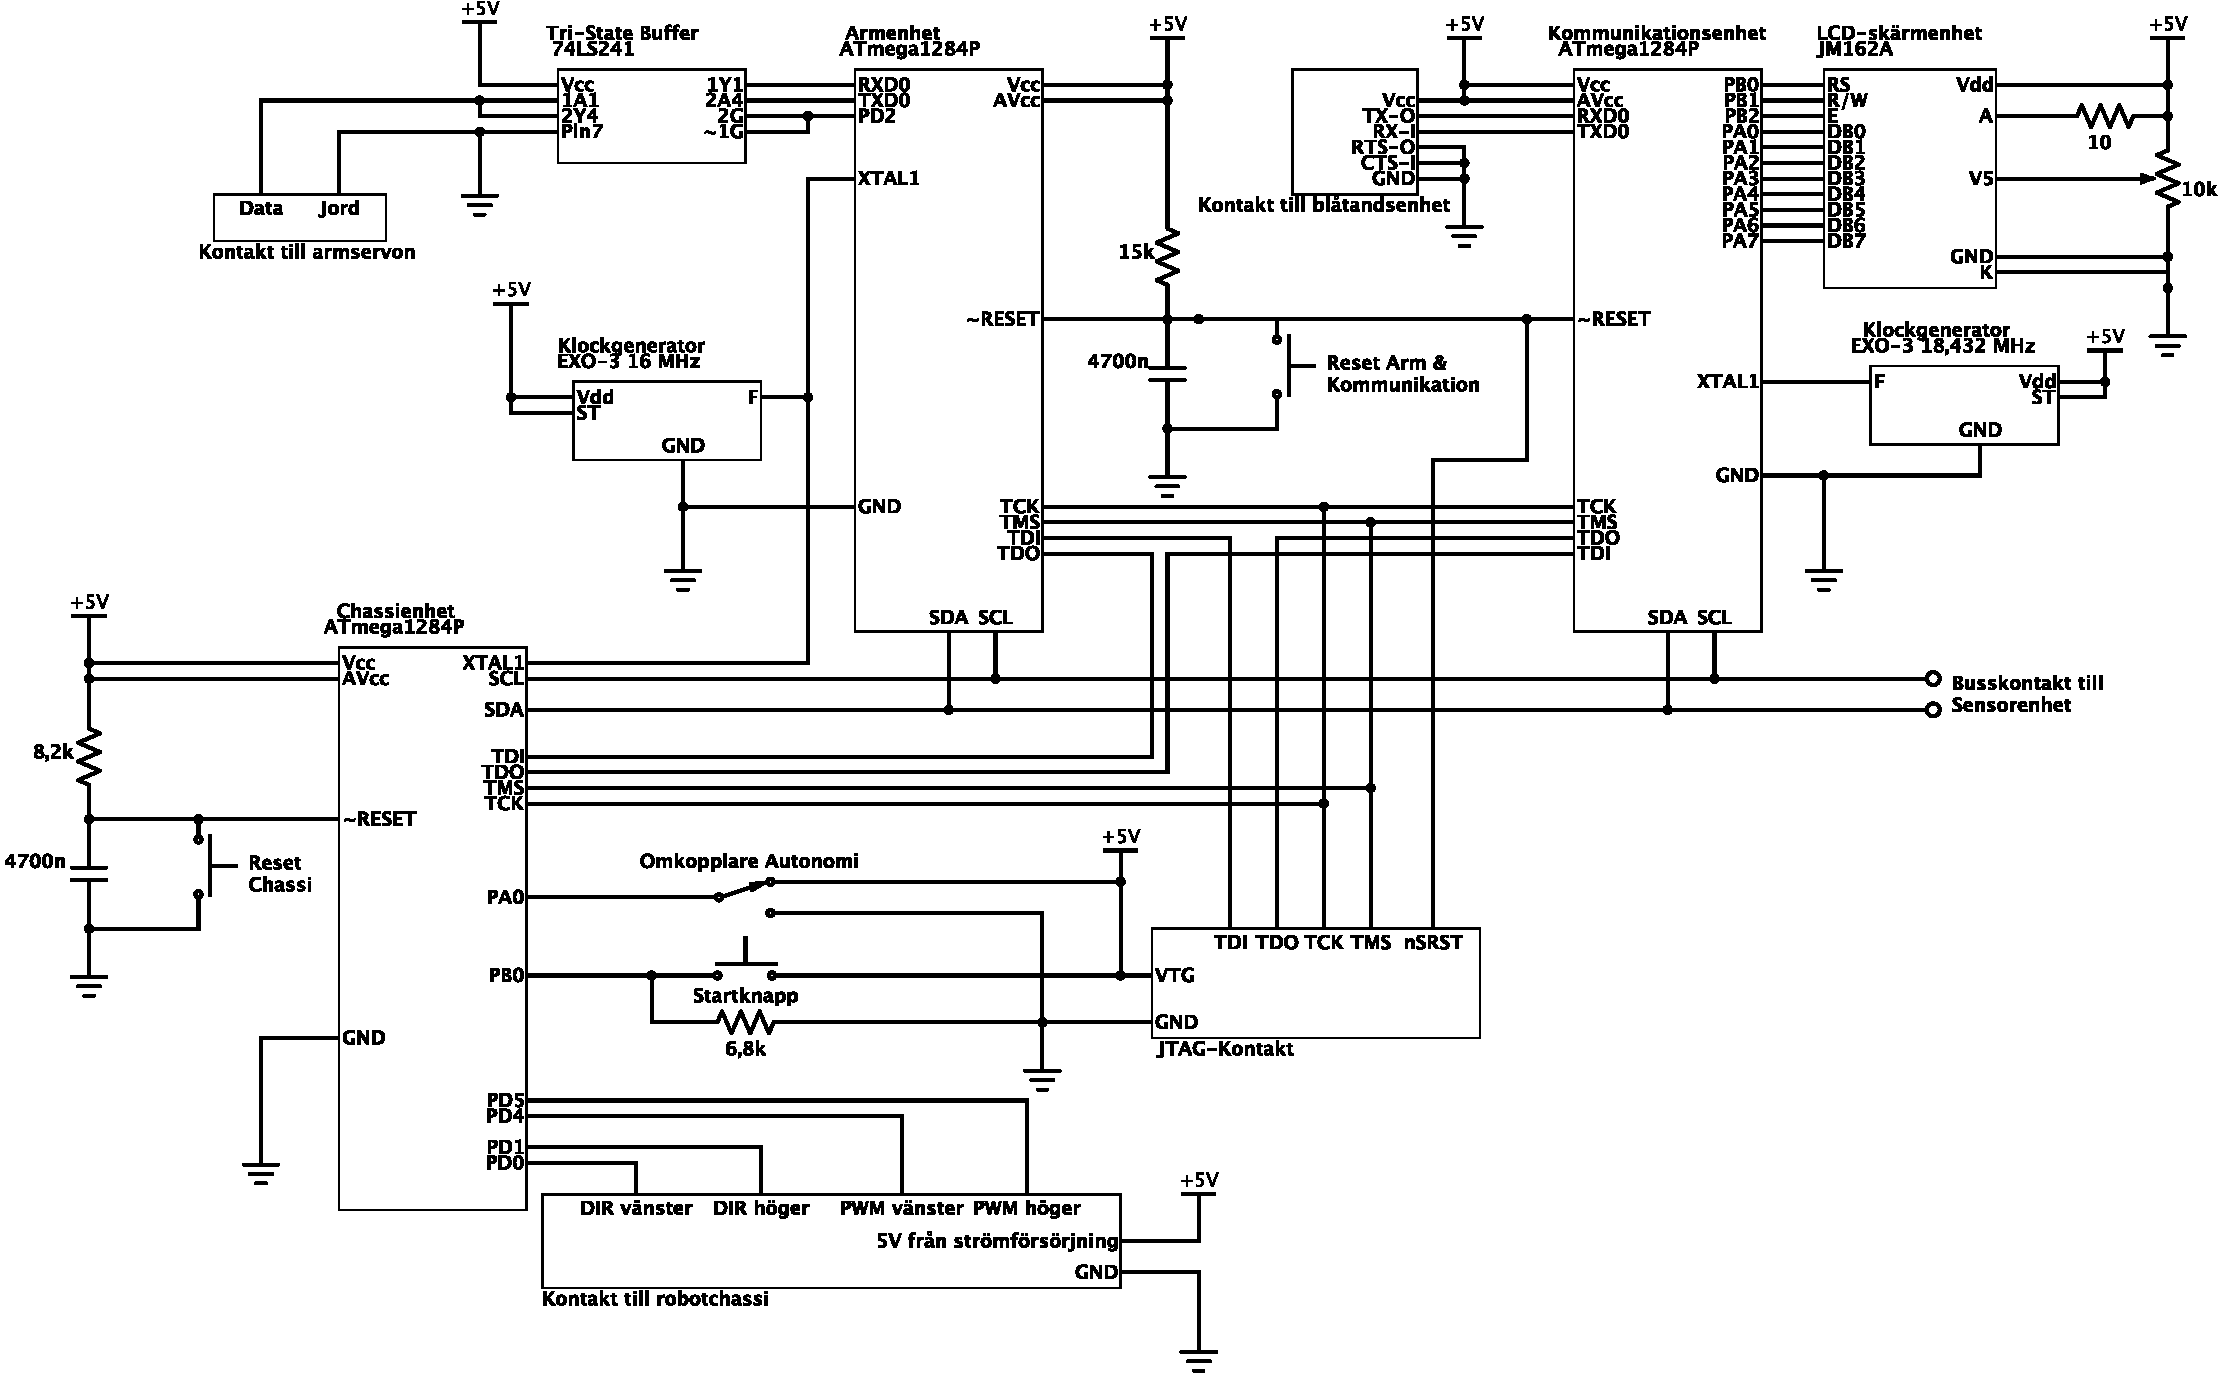
\includegraphics[angle=90,width=0.9\textwidth]{bilder/chassiarmkomm.pdf}
  \emph{\caption{Kopplingsschema över virkortet som innehåller kommunikationsenheten, chassienheten och armenheten.} \label{fig:chassiarmkomm}}
  
\end{figure}


\section{Utdrag från programlistning}
\emph{(ca 5-10 sidor så att vi kan bedöma kodens läsbarhet mm.) och eventuell VHDL-kod}
\section{Övriga bilagor?}


\end{document} 
